%%%%%%%%%%%%%%%%%%%%%%%%%%%%%%%%%%%%%%%%%%%%%%%%%%%%%%%%%%%%%%%%
%%%%%%%%%%%%%%%%%%%%%%%%%%%%%%%%%%%%%%%%%%%%%%%%%%%%%%%%%%%%%%%%
%%%%
%%%% This text file is part of the source of slides for
%%%% `The Art of HPC, vol 1: The Science of Computing'
%%%% by Victor Eijkhout, copyright 2012-2020
%%%%
%%%%%%%%%%%%%%%%%%%%%%%%%%%%%%%%%%%%%%%%%%%%%%%%%%%%%%%%%%%%%%%%
%%%%%%%%%%%%%%%%%%%%%%%%%%%%%%%%%%%%%%%%%%%%%%%%%%%%%%%%%%%%%%%%

\newcommand\repr{\mathop{\mathrm{rep}}}
\newcommand\intr{\mathop{\mathrm{int}}}

\begin{numberedframe}{Numbers in scientific computing}
\begin{itemize}
\item Integers: $\ldots,-2,-1,0,1,2,\ldots$
\item Rational numbers: $1/3,22/7$: not often encountered
\item Real numbers $0,1,-1.5,2/3,\sqrt 2,\log 10,\ldots$
\item  Complex numbers $1+2i,\sqrt 3-\sqrt 5i,\ldots$
\end{itemize}

Computers use a finite number of bits to represent numbers,\\
so only a finite number of numbers can be represented, and 
no irrational numbers (even some rational numbers).
\end{numberedframe}

\Level 1 {First we dig into bits}

\begin{numberedframe}{Bit operations}
\begin{tabular}{rllll}
  \toprule
  &boolean&bitwise (C)&bitwise (F)&bitwise (Py)\\
  and&\verb+&&+ & \verb+&+ & \n{iand} & \verb+&+ \\
  or &\verb+||+ & \verb+|+ & \n{ior}  & \verb+|+ \\
  not&\verb+!+  &          &          & \verb+~+ \\
  xor&          & \verb+^+ & \n{ieor} &          \\
  \bottomrule
\end{tabular}

Bit shift operations in~C:

\begin{tabular}{rl}
  \toprule
  left  shift& \verb+<<+ \\
  right shift& \verb+>>+ \\
  \bottomrule
\end{tabular}

Fortran: \n{mvbits}

\end{numberedframe}

\begin{numberedframe}{Arithmetic with bit ops}
  \begin{itemize}
  \item Left-shift is multiplication by~2:\\
\begin{lstlisting}
i_times_2 = i<<1;
\end{lstlisting}
\item Extract bits:
\begin{lstlisting}
i_mod_8 = i & 7
\end{lstlisting}
(How does that last one work?)
  \end{itemize}

\end{numberedframe}

\begin{exercise}{Bit operations}
  \label{ex:bit-even}
  Use bit operations to test whether a number is odd or even.\\
  Can you think of more than one way?
\end{exercise}

\Level 1 {Integers}

\begin{numberedframe}{Integers}
Scientific computation mostly uses real numbers. Integers
are mostly used for array indexing.

We look at
\begin{enumerate}
\item integers as supported by the hardware;
\item integers as they exist in programming languages;
\item (and not software-defined integers)
\end{enumerate}
\end{numberedframe}

\begin{numberedframe}{In C/C++ and Fortran}
  C:
\begin{itemize}
\item A short int is at least 16 bits;
\item An integer is at least 16 bits, but often 32 bits;
\item A long integer is at least 32 bits, but often~64;
\item A \indextermttdef{long long} integer is at least 64 bits.
\end{itemize}

Fortran uses kinds, not necessarily equal to number of bytes:
\lstset{language=Fortran}
\begin{lstlisting}
  integer(2) :: i2
  integer(4) :: i4
  integer(8) :: i8  
\end{lstlisting}
Specify the number of decimal digits with \n{selected_int_kind(n)}.
\lstset{language=C}

\end{numberedframe}

\begin{exercise}{Powers of two}
  \label{ex:two-powers}
  Print $2^n$ for $n=0,\ldots,31$. There are at least two ways of
  generating these powers.

  Also print the bit pattern. What is unexpected?
\end{exercise}

\begin{numberedframe}{Negative integers}
  Problem:
  \begin{itemize}
  \item How do we represent them?
  \item How do we do efficient arithmetic on them?
  \end{itemize}
  Define
  \[ \repr\colon {\cal Z}\rightarrow 2^n \]
  `representation of the number $N\in{\cal Z}$ as bitstring of length~$n$.'
  \[ \intr\colon 2^n \rightarrow {\cal Z} \]
  `interpretation of the bitstring of length~$n$ as number $N\in{\cal Z}$'
\end{numberedframe}

\begin{numberedframe}{Negative integers}
Use of sign bit: typically first bit

\[
\begin{array}{|r|r|}
  \hline
  s&i_1\ldots i_n\\ \hline
\end{array}
\]

Simplest solution:
\[
\begin{cases}
  n\geq 0&\repr(n)= 0,i_1,\ldots i_{31}\\
  n<0& \repr(-n)= 1,i_1,\ldots i_{31}
\end{cases}
\]
\end{numberedframe}

\begin{numberedframe}{Sign bit}
  Interpretation
  \[
\begin{array}{|c|rrrrrr|}
  \hline
  \hbox{bitstring}&
  00\cdots0&\ldots&01\cdots1&
  10\cdots0&\ldots&11\cdots1\\ \hline
  \hbox{as unsigned int}&
  0&\ldots&2^{31}-1&
  2^{31}&\ldots&2^{32}-1\\ \hline
  \hbox{as naive signed}&
  0&\ldots&2^{31}-1&
  -0&\ldots&-2^{31}+1\\ \hline
\end{array}
\]
\end{numberedframe}

\begin{numberedframe}{Shifting}
Interpret unsigned number $n$ as $n-B$
\[
\begin{array}{|c|rrrrrr|}
  \hline
  \hbox{bitstring}&
  00\cdots0&\ldots&01\cdots1&
  10\cdots0&\ldots&11\cdots1\\ \hline
  \hbox{as unsigned int}&
  0&\ldots&2^{31}-1&
  2^{31}&\ldots&2^{32}-1\\ \hline
  \hbox{as shifted int}&
  -2^{31}&\ldots&-1&
  0&\ldots&2^{31}-1\\ \hline
\end{array}
\]
\end{numberedframe}

\begin{numberedframe}{2's Complement}
  Let $m$ be a signed integer, then the 2's complement `bit pattern'
  $\repr(m)$ is a non-negative integer defined as follows:
  \begin{itemize}
  \item If $0\leq m\leq 2^{31}-1$, the normal bit pattern for $m$ is
    used, that is
    \[ 0\leq m\leq 2^{31}-1 \Rightarrow \repr(m) = m. \]
  \item For $-2^{31}\leq n\leq -1$, $n$ is represented by the bit
    pattern for $2^{32}-|n|$:
    \[ -2^{31}\leq n\leq -1 \Rightarrow \repr(m) = 2^{32}-|n|. \]
  \end{itemize}
\end{numberedframe}

\begin{numberedframe}{2's complement visualized}

  \[
  \begin{array}{|c|rrrrrr|}
    \hline
    \hbox{bitstring}&
    00\cdots0&\ldots&01\cdots1&
    10\cdots0&\ldots&11\cdots1\\ \hline
    \hbox{as unsigned int}&
    0&\ldots&2^{31}-1&
    2^{31}&\ldots&2^{32}-1\\ \hline
    \hbox{as 2's comp. integer}&
    0&\cdots&2^{31}-1&
    -2^{31}&\cdots&-1\\
    \hline
  \end{array}
  \]
\end{numberedframe}

\begin{numberedframe}{Integer arithmetic}
  Problem: processor is very good at artithmetic on (unsigned) bit strings.

  How does that translate to arithmetic on integers?

  \[ \intr\left( \repr(x) \mathop{*} \repr(y) \right)
        \mathrel{\overset{\makebox[0pt]{\mbox{\normalfont\tiny\sffamily ?}}}{=}}
      x \mathop{*} y
  \]

\end{numberedframe}

\begin{numberedframe}{Addition in 2's complement}
Add $m+n$, where $m,n$ are representable:
\[ 0\leq |m|,|n|<2^{31}. \]

 The easy case is $0<m,n$, as long as there is no overflow.
\end{numberedframe}

\begin{numberedframe}{Addition in 2's complement (cont'd)}
 Case $m>0$, $n<0$, and $m+n>0$. 
  Then $\repr(m)=m$ and
  $\repr(n)=2^{32}-|n|$, so the unsigned addition becomes
  \[ \repr(m)+\repr(n)=m+(2^{32}-|n|)=2^{32}+m-|n|. \]
  Since $m-|n|>0$, this result is~$>2^{32}$.
  %
  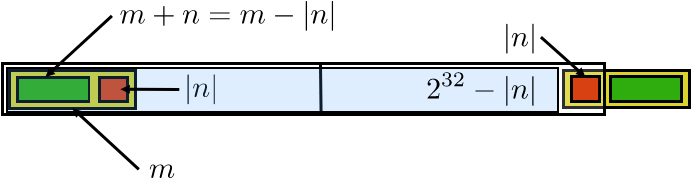
\includegraphics[scale=.4]{mminusn1}
  %
  However, this is basically $m+n$ with the overflow bit set.
\end{numberedframe}

\begin{numberedframe}{Subtraction in 2's complement}
Subtraction $m-n$:
\begin{itemize}
\item Case: $m<n$. Observe that $-n$ has the bit pattern of $2^{32}-n$.
  Also, $m+(2^{32}-n)=2^{32}-(n-m)$ where $0<n-m<2^{31}-1$,
  so $2^{32}-(n-m)$ is the 2's complement bit pattern of $m-n$.
\item Case: $m>n$.  The bit pattern for $-n$ is $2^{32}-n$, so
  $m+(-n)$ as unsigned is $m+2^{32}-n=2^{32}+(m-n)$. Here
  $m-n>0$. The $2^{32}$ is an overflow bit; ignore.
\end{itemize}
\end{numberedframe}

\begin{numberedframe}{Overflow}
  There is a limited number of bits, so numbers that are too large in
  absolute value can not be represented.

  Overflow.

  This is not a fatal error: your program continues with the wrong result.
\end{numberedframe}

\begin{exercise}{Integer overflow}
  Investigate what happens when you perform an integer calculation
  that leads to overflow. What
  does your compiler say if you try to write down a nonrepresentible
  number explicitly, for instance in a declaration or assignment statement?

  Language lawyer remark: signed integer overflow is Undefined Behavior in C/C++.
\end{exercise}

\Level 1 {Floating point numbers}

\renewcommand\repr{\mathop{\mathrm{fl}}}

\begin{numberedframe}{Floating point math is hard!}
  And the consequences if you get it wrong can be considerable.
  
  
\includegraphics[scale=.15]{race-nan}
\end{numberedframe}

\begin{numberedframe}{Floating point numbers}

Analogous to scientific notation $x=6.022\cdot 10^{23}$:
\[ x = \pm \Sigma_{i=0}^{t-1} d_i\beta^{-i} \, \beta^e \]
\begin{itemize}
\item sign bit
\item $\beta$ is the base of the number system
\item $0\leq d_i\leq \beta-1$ the digits of the \emph{mantissa}:\\
  one digit before the \emph{radix point}, so mantissa~$<\beta$
\item $e\in [L,U]$ exponent, stored with bias: unsigned int where
  $\repr(L)=0$
\end{itemize}
\end{numberedframe}

\begin{numberedframe}{Examples of floating point systems}

  \begin{tabular}{rrrrr}
    \toprule
    &$\beta$&$t$&$L$&$U$\\
    \midrule
    IEEE single (32 bit)&2&23&-126&127\\
    IEEE double (64 bit)&2&53&-1022&1023\\
    Old Cray 64bit&2&48&-16383&16384\\
    IBM mainframe 32 bit&16&6&-64&63\\
    packed decimal&10&50&-999&999\\
    \bottomrule
  \end{tabular}
  
  BCD is tricky: 3 decimal digits in 10 bits

  (we will often use $\beta=10$ in the examples, because it's easier to
  read for humans, but all practical computers use $\beta=2$)

  Internal processing in 80 bit
\end{numberedframe}

\begin{numberedframe}{Limitations}
  Overflow:
  more than $\beta(1-\beta^{-t+1}) \beta^U$ or less than
  $-\beta(1-\beta^{-t+1}) \beta^U$

  Underflow: positive numbers less than $\beta^L$\\
  Gradual underflow: $\beta^{-t+1}\cdot \beta^L$\\

  Overflow leads to \texttt{Inf}.
\end{numberedframe}


\begin{exercise}{Floating point overflow}
  For real numbers $x,y$, the quantity $g=\sqrt{(x^2+y^2)/2}$ satisfies
  \[ g\leq \max\{|x|,|y|\} \]
  so it is representable if $x$ and~$y$ are.
  What can go wrong if you compute $g$ using the above formula?
  Can you think of a better way?
\end{exercise}

\begin{numberedframe}{Other exceptions}
  Overflow: \texttt{Inf}

  \texttt{Inf}$-$\texttt{Inf}$\rightarrow$\texttt{NaN}\\
  also $0/0$ or $\sqrt{-1}$

  This does not stop your program in general\\
  sometimes possible
\end{numberedframe}

\begin{numberedframe}{The normalization problem}
  Do we allow
  \[ 1.100\cdot 10^{0},\quad 0.110\cdot 10^1,\quad 0.011\cdot
  10^{2}? \]
  This makes testing for equality hard.

  Solution: normalized numbers have one nonzero before the radix point.
\end{numberedframe}

\begin{numberedframe}{Normalized floating point numbers}

Require first digit in the mantissa to be nonzero.\\
Equivalent: mantissa part $1\leq x_m<\beta$

Unique representation for each number,\\
also: in binary this makes the first digit~1, so we don't need to
store that.\\
(do you see a problem?)

With normalized numbers, underflow threshold is
$1\cdot\beta^L$;\\
`gradual underflow' possible, but usually not efficient.
\end{numberedframe}

\begin{numberedframe}{IEEE 754, 32-bit pattern}
\small
  \[
  \begin{array}{| l || l || l |}
    \hline
    \hbox{sign}&\hbox{exponent}&\hbox{mantissa}\\
    \hline
    p&e=e_1\cdots e_8 &s=s_1\dots s_{23}\\
    \hline
    31&30\cdots 23&22\cdots 0\\
    \hline
    \pm & 2^{e-127} & s_1\cdot 2^{-1}+\cdots + s_{23}\cdot 2^{-23} \\
    & \hbox{(except $e=0,255$)} & \\
    \hline
  \end{array}\quad
  \]
\end{numberedframe}

\begin{numberedframe}{IEEE 754, 32-bit, all cases}
  \scriptsize
  \[
  \begin{array}{|r|r|l|}
    \hline
    (e_1\cdots e_8)&\hbox{numerical value}&\hbox{range}\\
    \hline
    (0\cdots0)=0& \pm 0.s_1\cdots s_{23}\times 2^{-126}
            &s=0\cdots 01\Rightarrow 2^{-23}\cdot 2^{-126}=2^{-149}\approx 10^{-45}\\
    &       &s=1\cdots 11\Rightarrow (1-2^{-23})\cdot 2^{-126}\\
    \hline
    (0\cdots 01)=1& \pm 1.s_1\cdots s_{23}\times 2^{-126}
            &s=0\cdots 01\Rightarrow 1 \cdot 2^{-126}\approx 10^{-37}\\
    \hline
    (0\cdots 010)=2& \pm 1.s_1\cdots s_{23}\times 2^{-125}&\\
    \hline
    \cdots&&\\
    \hline
    (01111111)=127 & \pm 1.s_1\cdots s_{23}\times 2^{0}
            &s=0\cdots 00\Rightarrow 1\cdot 2^{0}=1\\
    &       &s=0\cdots 01\Rightarrow 1+2^{-23}\cdot 2^{0}=1+\epsilon\\
    &       &s=1\cdots 11\Rightarrow (2-2^{-23})\cdot 2^{0}=2-\epsilon\\
    \hline
    (10000000)=128 & \pm 1.s_1\cdots s_{23}\times 2^{1}
            &s=0\cdots 00\Rightarrow 1\cdot 2^{1}=2\\
    \hline
    \cdots&
            &\hbox{et cetera}\\
    \hline
    (11111110)=254 & \pm 1.s_1\cdots s_{23}\times 2^{127}&\\
    \hline
    (11111111)=255 & s_1\cdots s_{23}=0 \Rightarrow \pm\infty &\\
                   & s_1\cdots s_{23}\not=0 \Rightarrow \n{NaN} &\\
    \hline
  \end{array}
  \]
\end{numberedframe}

\begin{exercise}{Float vs Int}
  Note that the exponent doesn't come at the end. This has an interesting consequence.

  What is the interpretation of
  \[ 0\cdots 0\,1\,1\,1 \]
  as int? What as float?

  What is the largest integer that is representible as float?
\end{exercise}

\begin{numberedframe}{Other precisions}
  \begin{itemize}
  \item There is a 64-bit format, with 53 bits mantissa.
  \item IEEE envisioned a sliding scale of precisions: see Intel 80-bit
    registers
  \item Half precision, and recent invention \n{bfloat16}
  \end{itemize}
  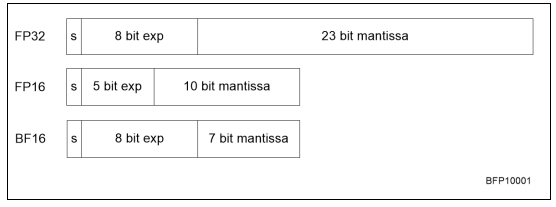
\includegraphics[scale=.4]{bfloat16def}  
\end{numberedframe}

\Level 1 {Floating point math}

\begin{numberedframe}{Representation error}
Error between number $x$ and representation~$\tilde x$:\\
absolute $x-\tilde x$ or $|x-\tilde x|$\\
relative $\frac{x-\tilde x}{x}$ or $\left|\frac{x-\tilde x}{x}\right|$

Equivalent: $\tilde x=x\pm\epsilon\Leftrightarrow |x-\tilde
x|\leq\epsilon \Leftrightarrow \tilde x\in[x-\epsilon,x+\epsilon]$.

Also: $\tilde x =x(1+\epsilon)$ often shorthand for
$\left|\frac{\tilde x-x}{x}\right|\leq \epsilon$
\end{numberedframe}

\begin{numberedframe}{Example}
Decimal, $t=3$ digit mantissa: let $x=1.256$, $\tilde
x_{\mathrm{round}}=1.26$, $\tilde x_{\mathrm{truncate}}=1.25$

Error in the 4th digit.\\
Different story for decimal vs binary.

How would this story change with a non-zero exponent,\\
for instance $1.256\cdot 10^{12}$?
\end{numberedframe}


\begin{exercise}{Round-off}
  \input{ex:e-compute}
%%   The number $e\approx 2.72$, the base for the natural logarithm, has
%%   various definitions. One of them is 
%%   \[ e=\lim_{n\rightarrow\infty} (1+1/n)^n. \]
%%   Write a single precision program that tries to compute~$e$ in this
%%   manner. Evaluate the expression for an upper bound $n=10^k$ with
%%   $k=1,\ldots,10$. Explain the output for large~$n$. Comment on the
%%   behavior of the error.

%%   Can you come up with a better way of computing~$e$?
%%   How is this number actually computed?
\end{exercise}
\begin{answer}
  \snippetwithoutput{elimit}{code/754}{elimit}
\end{answer}

\begin{numberedframe}{Machine precision}
  Any real number can be represented to a certain precision:
  %
  $\tilde x=x(1+\epsilon)$ where\\
  truncation: $\epsilon=\beta^{-t+1}$\\
  rounding: $\epsilon=\frac12 \beta^{-t+1}$

  This is called \emph{machine precision}: maximum relative error.

  32-bit single precision: $mp\approx10^{-7}$\\ \relax
  64-bit double precision: $mp\approx10^{-16}$
  
  Maximum attainable accuracy.
  
  Another definition of machine precision: smallest number $\epsilon$ such that
  $1+\epsilon>1$.
\end{numberedframe}

\begin{exercise}{Machine epsilon}
  Write a small program that computes the machine epsilon for both
  single and double precision. Does it
  make any difference if you set the
  \indextermbus{compiler}{optimization levels} low or high? 

  (For C++ programmers: can you write a templated program that works
  for single and double precision?)
\end{exercise}

\begin{numberedframe}{Addition}
  \begin{enumerate}
  \item align exponents
  \item add mantissas
  \item adjust exponent to normalize
  \end{enumerate}

Example: $1.00+2.00\times 10^{-2}=1.00+.02=1.02$. This is exact, but
what happens with $1.00+2.55\times 10^{-2}$?

Example: $5.00\times 10^{1}+5.04=(5.00+0.504)\times10^1
\rightarrow5.50\times10^1$

Any error comes from limiting the mantissa: if $x$ is the true sum
and $\tilde x$ the computed sum, then $\tilde x=x(1+\epsilon)$ with 
$|\epsilon|<10^{-2}$
\end{numberedframe}

\begin{numberedframe}{The `correctly rounded arithmetic' model}
Assumption (enforced by IEEE 754):
\begin{quotation}
  The numerical result of an operation is the rounding of the exactly
  computed result.
\end{quotation}
\[ \repr(x_1\odot x_2) = (x_1\odot x_2)(1+\epsilon) \]
where $\odot=+,-,*,/$

Note: this holds only for a single operation!
\end{numberedframe}

\begin{numberedframe}{Guard digits}
Correctly rounding is not trivial, especially for subtraction.

Example: $t=2, \beta=10$: $1.0-9.5\times 10^{-1}$, exact result
$0.05=5.0\times 10^{-2}$.
\begin{itemize}
\item Simple approach: $1.0-9.5\times 10^{-1}=1.0-0.9=0.1=1.0\times
  10^{-1}$
\item Using `guard digit': $1.0-9.5\times
  10^{-1}=1.0-0.95=0.05=5.0\times 10^{-2}$, exact.
\end{itemize}
In general 3 extra bits needed.
\end{numberedframe}

\begin{numberedframe}{Fused Mul-Add instructions}
  (also `fused multiply-accumulate')
  \[ c\leftarrow a*b+c \]
  \begin{itemize}
  \item Addition plus multiplication, but not independent
  \item Processors can have dedicated hardware for FMA (also IEEE
    754-2008)
  \item Internally evaluated in higher precision: 80-bit.
  \item Very useful for certain linear algebra (which?) Not for other
    operations (examples?)
  \end{itemize}
  
\end{numberedframe}

\begin{numberedframe}{Associativity}
  Computate $4+6+7$ in one significant digit.
  
Evaluation left-to-right gives:
\[ 
\begin{array}{l@{{}\Rightarrow{}}lp{3in}}
(4\cdot10^0 + 6\cdot10^0)+7\cdot10^0&10\cdot10^0+7\cdot10^0&addition\\
&1\cdot 10^1 + 7\cdot10^0&rounding\\
&1.0\cdot 10^1 + 0.7\cdot10^1&using guard digit\\
&1.7\cdot 10^1\\
&2\cdot10^1&rounding
\end{array}
\]
On the other hand, evaluation right-to-left gives:
\[ 
\begin{array}{l@{{}\Rightarrow{}}lp{3in}}
4\cdot10^0 + (6\cdot10^0 + 7\cdot10^0)&4\cdot 10^0 + 13\cdot10^0&addition\\
&4\cdot 10^0 + 1\cdot10^1&rounding\\
&0.4\cdot 10^1 + 1.0\cdot10^1&using guard digit\\
&1.4\cdot 10^1\\
&1\cdot10^1&rounding
\end{array}
\]
\end{numberedframe}

\begin{numberedframe}{Error propagation under addition}
Let $s=x_1+x_2$, and $x=\tilde s=\tilde x_1+\tilde x_2$
with $\tilde x_i=x_i(1+\epsilon_i)$
\begin{eqnarray*}
\tilde x&=&\tilde s(1+\epsilon_3)\\
&=&x_1(1+\epsilon_1)(1+\epsilon_3)+x_2(1+\epsilon_2)(1+\epsilon_3)\\
&=&x_1+x_2+x_1(\epsilon_1+\epsilon_3)+x_2(\epsilon_2+\epsilon_3)\\
\Rightarrow\tilde x&=&s(1+2\epsilon)
\end{eqnarray*}
$\Rightarrow$ errors are added

Assumptions: all $\epsilon_i$ approximately equal size and small;\\
$x_i>0$
\end{numberedframe}

\begin{numberedframe}{Multiplication}
  \begin{enumerate}
  \item add exponents
  \item multiply mantissas
  \item adjust exponent
  \end{enumerate}

Example: $.123\,\times\,.567\times10^1=.069741\times10^1\rightarrow
.69741\times10^0\rightarrow.697\times10^0$.

What happens with relative errors?
\end{numberedframe}

\Level 1 {Examples}

\begin{numberedframe}{Subtraction}
Correct rounding only applies to a single operation.

Example: $1.24-1.23=0.01\rightarrow 1.\times 10^{-2}$:\\
result is exact, but only one significant digit.

What if $1.24=\repr(1.244)$ and $1.23=\repr(1.225)$? Correct
result~$1.9\times 10^{-2}$; almost 100\% error.
\begin{itemize}
\item \emph{Cancellation} leads to loss of precision
\item subsequent operations with this result are inaccurate
\item this can not be fixed with guard digits and such
\item $\Rightarrow$ avoid subtracting numbers that are likely close.
\end{itemize}
\end{numberedframe}

\begin{numberedframe}{ABC-formula}
  Example: $ax^2+bx+c=0\rightarrow x=\frac{-b\pm\sqrt{b^2-4ac}}{2a}$\\
  suppose $b>0$ and $b^2\gg 4ac$ then the `$+$' solution will be
  inaccurate\\
  Better: compute $x_-=\frac{-b-\sqrt{b^2-4ac}}{2a}$ and use $x_+\cdot
  x_-=-c/a$.
\end{numberedframe}

\begin{numberedframe}{Serious example}
  \small

Evaluate $\Sigma_{n=1}^{10000}\frac{1}{n^2}=1.644834$ \\
in 6 digits: machine precision is $10^{-6}$ in single precision

First term is 1, so partial sums are $\geq1$, so $1/n^2<10^{-6}$ gets
ignored,
$\Rightarrow$ last 7000 terms (or more) are ignored,
$\Rightarrow$ sum is $1.644725$: 4 correct digits

Solution: sum in reverse order; exact result in single precision\\
Why? Consider ratio of two terms:
\[ \frac{n^2}{(n-1)^2}=\frac{n^2}{n^2-2n+1}=\frac1{1-2/n+1/n^2}
    \approx 1+\frac2n
\]
with aligned exponents:\\
\begin{tabular}{rrcl}
  $n-1$:&$.00\cdots0$&$10\cdots00$\\
  $n$:&  $.00\cdots0$&$10\cdots01$&$0\cdots0$\\
      &             &\multicolumn{2}{l}{$k=\log(n/2)$ positions}
\end{tabular}

The last digit in the smaller number is not lost if $n<2/\epsilon$
\end{numberedframe}

\begin{numberedframe}{Another serious example}
\small
Previous example was due to finite representation; this example is
more due to algorithm itself.

Consider $y_n=\int_0^1 \frac{x^n}{x-5}dx = \frac1n-5y_{n-1}$
(monotonically decreasing)\\
$y_0=\ln 6 - \ln 5$.

In 3 decimal digits:\\
\begin{tabular}{lll}
  computation&&correct result\\
  $y_0=\ln 6 - \ln 5=.182|322\times 10^{1}\ldots$&&1.82\\
  $y_1=.900\times 10^{-1}$&&.884\\
  $y_2=.500\times 10^{-1}$&&.0580\\
  $y_3=.830\times 10^{-1}$&going up?&.0431\\
  $y_4=-.165$&negative?&.0343
\end{tabular}

Reason? Define error as $\tilde y_n=y_n+\epsilon_n$, then
\[ \tilde y_n=1/n-5\tilde y_{n-1}=1/n+5n_{n-1}+5\epsilon_{n-1}
    = y_n+5\epsilon_{n-1} \]
so $\epsilon_n\geq 5\epsilon_{n-1}$: exponential growth.
\end{numberedframe}

\begin{numberedframe}{Stability of linear system solving}

Problem: solve $Ax=b$, where $b$ inexact.
\[ A(x+\Delta x)=b+\Delta b. \]
Since $Ax=b$, we get $A\Delta x=\Delta b$. From this,
\[
 \left \{
\begin{array}{rl}
  Ax&=b\\ \Delta x&=A\inv \Delta b\\ 
\end{array} \right\} \Rightarrow \left\{
\begin{array}{rl}
  \|A\| \|x\|&\geq\|b\| \\ \|\Delta x\|&\leq \|A\inv\| \|\Delta b\|
\end{array} \right.
\]
\[
\Rightarrow
\frac{\|\Delta x\|}{\|x\|}
\leq 
\|A\| \|A\inv\| \frac{\|\Delta b\|}{\|b\|}
\]
`Condition number'. Attainable accuracy depends on matrix properties
\end{numberedframe}

\begin{numberedframe}{Consequences of roundoff}

Multiplication and addition are not associative:\\
problems for parallel computations.

\begin{tabular}{cc}
  \midrule
  \multicolumn{2}{c}{compute $a+b+c+d$}\\
  sequential&parallel\\
  \midrule
  $((a+b)+c)+d$&(a+b)+(c+d)\\
  \midrule
\end{tabular}

Operations with ``same'' outcomes are not equally stable:\\
matrix inversion is unstable, elimination is stable
\end{numberedframe}

\begin{exercise}{Fixed-point iteration}
  Consider the iteration
  \[ x_{n+1}=f(x_n) = \
  \begin{cases}
    2x_n&\hbox{if $2x_n<1$}\\
    2x_n-1&\hbox{if $2x_n\geq 1$}\\
  \end{cases}
  \]
  Does this function have a fixed point, $x_0\equiv f(x_0)$, or is there a cycle
  $x_1=f(x_0),\,x_0\equiv x_2=f(x_1)$ et cetera?

  Now code this function and see what happens with various starting
  points~$x_0$. Can you explain this?
\end{exercise}

\Level 1 {More}

\begin{numberedframe}{Complex numbers}
Two real numbers: real and imaginary part.

Storage:
\begin{itemize}
\item Store real/imaginary adjacent: easy to pass address of one
  number
\item Store array of real, then array of imaginary. Better for
  stride~1 access if only real parts are needed. Other considerations.
\end{itemize}
\end{numberedframe}

\begin{numberedframe}{Other arithmetic systems}
Some compilers support higher precisions.

Arbitrary precision: GMPlib

Interval arithmetic

Half precision bfloat16
\end{numberedframe}


